\documentclass[11pt,a4paper]{article}

% --- Essential Packages ---
\usepackage[margin=1.0in]{geometry}
\usepackage{amsmath,amssymb,amsfonts,amsthm}
\usepackage{booktabs}
\usepackage{graphicx}
\usepackage{hyperref}
\usepackage{url}
\usepackage{algorithm}
\usepackage{algorithmic}
\usepackage{microtype}
\usepackage{xcolor}
\usepackage{tabularx}
\usepackage{subcaption}
\usepackage{enumitem}
\usepackage{cite}

% --- Hyperref Setup ---
\hypersetup{
    colorlinks=true,
    linkcolor=blue!70!black,
    citecolor=green!50!black,
    urlcolor=blue!80!black
}

% --- Theorem & Definition Environments ---
\newtheorem{definition}{Definition}
\newtheorem{axiom}{Axiom}
\newtheorem{proposition}{Proposition}

% --- Title & Metadata ---
\title{\textbf{CRBench: A Method-Agnostic, Resource-Aware Evaluation Framework for Long-Context Large Language Models}}

\author{
  \textbf{Om Chimurkar} \quad \textbf{CRBench Contributors} \\
  \texttt{omchimurkar10@gmail.com} \\
  \url{https://github.com/Omc12/CRBench}
}

\date{\textbf{Research Preprint --- Version 0.2.0 (Research Preview)} \\ August 2026}

\begin{document}

\maketitle

\begin{abstract}
As Large Language Models (LLMs) expand their context windows to tens and hundreds of thousands of tokens, the Key-Value (KV) cache becomes the primary operational bottleneck during autoregressive inference, consuming tens of gigabytes of GPU memory and severely limiting batch concurrency. While dozens of context compression paradigms have emerged---spanning KV quantization, attention-sink eviction, semantic token merging, low-rank projection, and latent state representations---existing evaluation methodology remains fragmented. Current long-context benchmarks assess downstream task accuracy in isolation without measuring memory consumption, while systems papers report compression ratios on unstandardized tasks without an anchored baseline. 

In this work, we present \textbf{CRBench} (\textit{Context Resource Benchmark}), a method-agnostic, query-level evaluation framework that quantifies how much contextual capability an LLM retains relative to the memory and system resources it consumes. CRBench defines the atomic evaluation primitive as the 4-tuple $(\mathcal{M}, q, \mathcal{R}_{\text{dense}}, \mathcal{A})$, evaluating each query pairwise against the base model's uncompressed FP16/BF16 dense reference. We define a reference-anchored quality retention metric $Q$, an analytical and physical resource efficiency metric $R_{\text{mem}}$, and a resource-aware Part~1 utility score $\mathcal{S}_{\text{res}} = \alpha Q + (1 - \alpha) R_{\text{mem}}$ (default $\alpha = 0.70$). We further specify a decoupled Part~2 system track incorporating Time-To-First-Token (TTFT), prefill latency, and decode throughput. We describe the complete architecture of CRBench v0.2.0, release an open-source extensible framework supporting custom adapters in under 50 lines of code, evaluate scoring desiderata across seven candidate formulations, and report preliminary validation on a $0.5\text{B}$-parameter open-weight model across five representative tasks. CRBench proposes an open, reproducible framework for navigating the contextual quality--memory efficiency Pareto frontier.
\end{abstract}

\noindent\textbf{Keywords:} Long-Context LLMs, KV Cache Compression, Resource-Aware Evaluation, Memory Efficiency, Benchmarking, Inference Systems.

\vspace{1.0em}
\noindent\fbox{
\parbox{0.96\textwidth}{
\small
\textbf{Status Note (Research Preview v0.2.0):} This manuscript is an academic preprint documenting the theoretical formulation, software architecture, query-level methodology, and preliminary small-model validation of CRBench. CRBench is an active research project; extensive empirical validation across 7B--8B+ parameter models and ultra-long sequences ($>32\text{K}$ tokens) is actively ongoing.
}
}
\vspace{1.0em}

% ==============================================================================
% 1. INTRODUCTION
% ==============================================================================
\section{Introduction}
\label{sec:introduction}

Modern Large Language Models (LLMs) have achieved remarkable breakthroughs across multi-document synthesis, extended multi-hop question answering, repository-scale code analysis, and complex agentic workflows~\cite{brown2020language,achiam2023gpt4,touvron2023llama,bai2023qwen}. These capabilities rely on long-context processing, expanding model context windows from 2,048 tokens to 32,768, 128,000, and even 1,000,000 tokens~\cite{reid2024gemini,deepseek2024v2}.

However, this contextual expansion is fundamentally bounded by the memory footprint of the Key-Value (KV) cache in standard Transformer architectures~\cite{vaswani2017attention}. Because standard self-attention caches intermediate key and value tensor representations for every token across all attention heads and layers, KV cache memory scales linearly with sequence length $L$ and batch size $B$:
\begin{equation}
\label{eq:kv_size_intro}
M_{\text{KV}} = 2 \times N_{\text{layers}} \times N_{\text{kv\_heads}} \times d_{\text{head}} \times L \times B \times \text{sizeof}(\text{dtype}) \quad [\text{bytes}].
\end{equation}
For a representative 8-billion parameter model (e.g., Llama-3.1-8B~\cite{dubey2024llama3} with 32 layers, 8 Key-Value heads with Grouped-Query Attention, and head dimension 128 in 16-bit precision), a single batch-1 128K-token context sequence ($L = 131{,}072$) requires exactly $16.0\,\text{GiB}$ ($17.18\,\text{GB}$) of memory purely for the KV cache ($2 \times 32 \times 8 \times 128 \times 131{,}072 \times 2\,\text{bytes}$)---exceeding the model's static 16-bit parameter footprint ($\approx 15.0\,\text{GiB}$ / $16.1\,\text{GB}$) and exhausting the VRAM of standard consumer GPUs.

To alleviate this severe bottleneck, the research community has proposed a rich taxonomy of KV cache compression techniques:
\begin{enumerate}[leftmargin=*]
    \item \textbf{KV Cache Quantization}: Representing keys and values in low-precision numerical formats, such as FP8, INT8, INT4, or non-uniform 2-bit formats with per-channel or group-wise scaling~\cite{dettmers2022llmint8,hooper2024kvquant,liu2024kivi,zhang2024fp8}.
    \item \textbf{KV Cache Eviction \& Sparsification}: Dynamically discarding unimportant historical tokens based on attention score accumulation, sliding local windows, or attention sinks (e.g., StreamingLLM~\cite{xiao2023streamingllm}, SnapKV~\cite{li2024snapkv}, $\text{H}_2\text{O}$~\cite{zhang2023h2o}, Scissorhands~\cite{liu2023scissorhands}).
    \item \textbf{KV Cache Merging \& Clustering}: Combining spatially or semantically adjacent token vectors through temporal pooling, hierarchical clustering, or weighted centroids~\cite{ge2023model,zhang2024pyramidkv}.
    \item \textbf{Low-Rank \& Subspace Projection}: Projecting KV tensors into low-dimensional latent subspaces via principal component analysis, singular value decomposition, or learned linear projections~\cite{sharma2023truth,chen2024compressing}.
    \item \textbf{Dynamic \& Disentangled KV (DKV) Representations}: Factoring context memory into shared static subspace bases and sparse dynamic token updates.
\end{enumerate}

Despite this rapid algorithmic progress, an acute methodological gap exists: \textit{the field lacks a unified, method-agnostic, resource-aware evaluation benchmark}. Current long-context evaluation suites (e.g., Needle-In-A-Haystack~\cite{kamradt2023needle}, RULER~\cite{hsieh2024ruler}, LongBench~\cite{bai2023longbench}, LongBench~v2~\cite{bai2024longbenchv2}) are primarily designed to evaluate model capability under uncompressed dense representations rather than to standardize quality retention under varying memory constraints. Conversely, papers introducing compression algorithms report accuracy on idiosyncratic task subsets alongside theoretical compression ratios, without controlling for base model capability, metadata storage overheads, or query-level variance.

To resolve these challenges, we introduce \textbf{CRBench} (\textit{Context Resource Benchmark}), an open, extensible, and principled evaluation framework designed to quantify how much contextual capability an LLM retains for the memory and system resources it consumes. 

CRBench is \textit{not} an empirical bake-off designed to crown a single compression technique. Rather, it is a reusable benchmarking harness and scoring specification that researchers and practitioners can apply to evaluate any existing or novel context memory representation.

\paragraph{Core Contributions.} The primary contributions of this work are:
\begin{itemize}[leftmargin=*]
    \item \textbf{The Query-Level Evaluation Primitive}: We formulate benchmark evaluation around the atomic 4-tuple $(\mathcal{M}, q, \mathcal{R}_{\text{dense}}, \mathcal{A})$, pairing every compressed method evaluation directly against the identical model's uncompressed dense FP16 reference on the exact same prompt, reducing prompt-selection and base-model capability confounding.
    \item \textbf{Model-Relative Capability Normalization}: We specify a reference-anchored quality metric $Q \in [0, 100]$ that isolates contextual representation fidelity from the base model's intrinsic zero-shot strength, incorporating a dynamic range gate to prevent division instabilities on small or saturated models.
    \item \textbf{Explicit Analytical \& Physical Memory Accounting}: We formalize effective bits-per-element ($b_{\text{eff}}$) and memory efficiency $R_{\text{mem}}$, accounting not only for raw tensor payloads but also quantization scales, codebooks, eviction index bitmaps, and alignment overheads.
    \item \textbf{Desiderata-Based Scoring Utility Analysis}: We evaluate seven candidate utility formulations against five key measurement desiderata (quality monotonicity, resource monotonicity, boundedness, Pareto consistency, and low-quality penalty criteria), proposing the linear additive formulation $\mathcal{S}_{\text{res}} = \alpha Q + (1 - \alpha) R_{\text{mem}}$ (default $\alpha = 0.70$) as a transparent, non-destructive scoring formulation.
    \item \textbf{Two-Track Benchmark Separation}: We decouple Part~1 (algorithmic context representation efficiency) from Part~2 (hardware-dependent system latency, TTFT, and decode throughput), enabling pure theoretical comparisons alongside deployability profiles.
    \item \textbf{Open-Source Extensible Implementation}: We release the modular CRBench v0.2.0 Python package featuring custom adapter registration in under 50 lines of code, non-destructive score recomputation, transparent failure categorization, and preliminary validation on a $0.5\text{B}$-parameter open-weight model.
\end{itemize}

% ==============================================================================
% 2. MOTIVATION & RELATED WORK
% ==============================================================================
\section{Motivation \& Related Work}
\label{sec:motivation}

\subsection{Limitations of Current Evaluation Paradigms}
Existing approaches to evaluating long-context models and compression techniques suffer from three structural shortcomings, summarized in Table~\ref{tab:paradigms}:

\begin{table*}[t]
\centering
\small
\caption{\textbf{Comparison of Common Evaluation Paradigms and Capabilities Provided by CRBench.} Summary of dimensions captured across long-context accuracy benchmarks, synthetic needle tests, inference profilers, and CRBench.}
\label{tab:paradigms}
\begin{tabularx}{\textwidth}{lccccc}
\toprule
\textbf{Evaluation Paradigm} & \textbf{Quality} & \textbf{Memory} & \textbf{System Latency} & \textbf{Dense-Anchored} & \textbf{Query-Level Pairwise} \\
\midrule
Standard Long-Context (e.g. LongBench) & \checkmark & $\times$ & $\times$ & $\times$ & $\times$ \\
Synthetic Needle Tests (e.g. NIAH, RULER) & \checkmark & $\times$ & $\times$ & $\times$ & $\times$ \\
Inference Systems Profilers (e.g. vLLM) & $\times$ & \checkmark & \checkmark & $\times$ & $\times$ \\
Ad-hoc Compression Papers & \checkmark & $\triangle$ & $\triangle$ & $\times$ & $\times$ \\
\textbf{CRBench (This Work)} & \textbf{\checkmark} & \textbf{\checkmark} & \textbf{\checkmark} & \textbf{\checkmark} & \textbf{\checkmark} \\
\bottomrule
\end{tabularx}
\end{table*}

\begin{enumerate}[leftmargin=*]
    \item \textbf{Quality--Resource Disconnection}: Traditional benchmarks (e.g., L-Eval~\cite{an2023leval}, BAMBOO~\cite{dong2023bamboo}, InfiniteBench~\cite{zhang2024infinitebench}) measure accuracy without tracking memory. A method that achieves 90\% accuracy while consuming 16 bits per token is treated identically to a method achieving 90\% accuracy at 4 bits per token, despite the latter offering $4\times$ greater hardware efficiency.
    \item \textbf{Confounding Base Model Capability with Representation Quality}: Reporting absolute task accuracy confuses the model's fundamental reasoning capability with the efficiency of the KV compression algorithm. A weak compression technique applied to a 70B parameter model might achieve a higher absolute accuracy than a state-of-the-art compression method on an 8B model. By anchoring evaluations to each model's uncompressed dense execution on the same query, CRBench isolates representation efficiency.
    \item \textbf{Ignoring Metadata and System Overhead}: Many compression works claim theoretical 4-bit or 2-bit compression while omitting the memory required for scaling factors, outlier vectors, or eviction index tables. Furthermore, algorithms that save memory by executing uncoalesced memory reads or expensive CPU--GPU synchronization can severely degrade prefill latency (TTFT) and decode throughput.
\end{enumerate}

\subsection{Related Work in Context Compression \& Benchmarking}

\paragraph{Long-Context Synthetic and Realistic Benchmarks.}
Needle-In-A-Haystack (NIAH)~\cite{kamradt2023needle} popularized probing multi-depth single-fact retrieval. RULER~\cite{hsieh2024ruler} generalized NIAH to variable tracking, multi-needle aggregation, and high-entropy key-value association, revealing that many models claiming 32K or 128K context degrade dramatically beyond 8K tokens. LongBench~\cite{bai2023longbench} and LongBench~v2~\cite{bai2024longbenchv2} curated multi-task document QA, summarization, and synthetic reasoning tasks. These benchmarks are primarily designed to measure contextual capability rather than to standardize quality under varying memory representations.

\paragraph{KV Cache Compression Techniques.}
To address KV memory growth, KVQuant~\cite{hooper2024kvquant}, KIVI~\cite{liu2024kivi}, and QA-LoRA~\cite{han2024qalora} introduced per-channel and asymmetric 2-to-4-bit quantization. Eviction policies such as StreamingLLM~\cite{xiao2023streamingllm} demonstrated the critical importance of initial ``attention sinks'' combined with local rolling buffers. SnapKV~\cite{li2024snapkv} and $\text{H}_2\text{O}$~\cite{zhang2023h2o} select heavy-hitter key tokens during prefill. PyramidKV~\cite{zhang2024pyramidkv} allocates layer-wise dynamic budgets. Despite their individual merits, each paper evaluates on disparate task sets, distinct token budgets, and incomparable metrics. CRBench provides the common benchmarking infrastructure required to evaluate these techniques uniformly.

% ==============================================================================
% 3. PROBLEM DEFINITION & MATHEMATICAL FORMULATION
% ==============================================================================
\section{Problem Definition \& Mathematical Formulation}
\label{sec:problem_definition}

Figure~\ref{fig:framework_overview} illustrates the overall architecture of CRBench, depicting the dual execution branches, reference-anchored normalization, and decoupled scoring tracks.

\begin{figure*}[t]
\centering
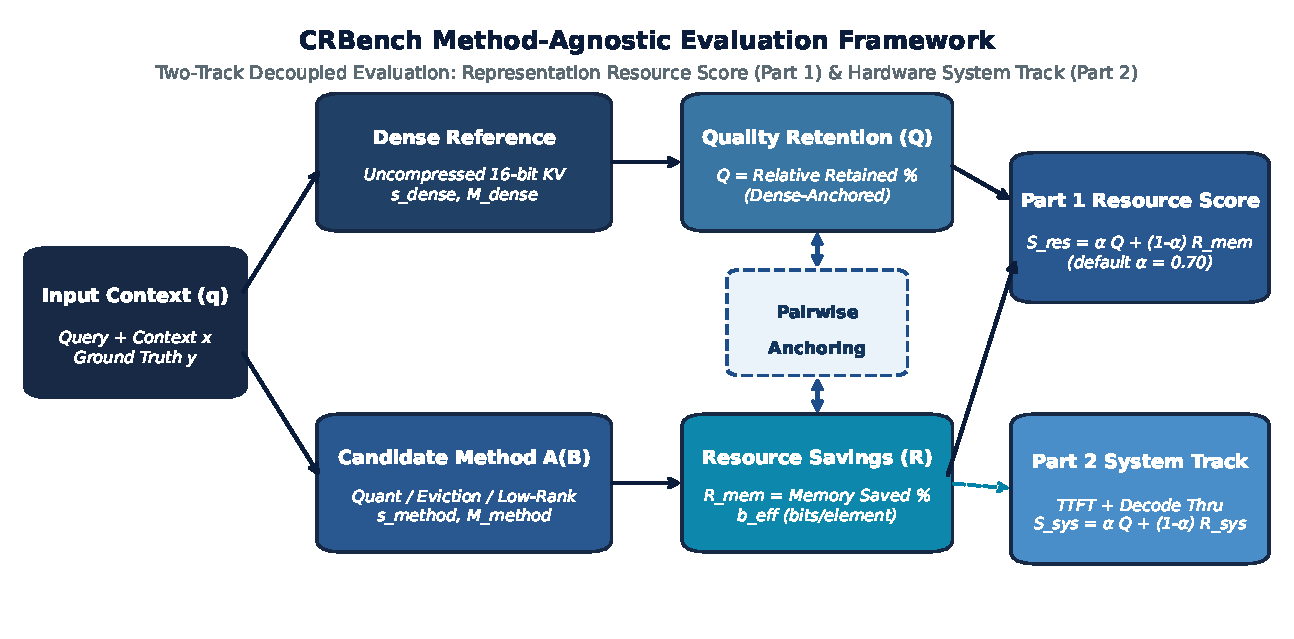
\includegraphics[width=0.96\textwidth]{tmlr/figures/fig1_framework_overview.pdf}
\caption{\textbf{CRBench Method-Agnostic Evaluation Framework Architecture.} The benchmark decouples evaluation into two complementary tracks: Part~1 (Algorithmic Representation Efficiency $\mathcal{S}_{\text{res}}$) and Part~2 (Hardware System Track $\mathcal{S}_{\text{sys}}$). Every candidate context representation $\mathcal{A}(\mathcal{B})$ is evaluated pairwise against the base model's uncompressed dense reference $\mathcal{R}_{\text{dense}}$ on the identical input query $(x_i, y_i)$.}
\label{fig:framework_overview}
\end{figure*}

\subsection{The Atomic Evaluation Primitive}
Let $\mathcal{M}$ denote an autoregressive language model parameterized by weights $\Theta$. An evaluation dataset $\mathcal{D} = \{(x_i, y_i, \tau_i, L_i)\}_{i=1}^N$ consists of queries $x_i$, ground-truth target outputs $y_i$, task types $\tau_i$, and prompt context token lengths $L_i$.

Let $\mathcal{A}$ denote a candidate context memory adapter (e.g., INT4 quantization or SnapKV eviction) operating under an assigned resource budget $\mathcal{B}$. In standard dense inference, the uncompressed reference adapter is denoted $\mathcal{R}_{\text{dense}}$ (16-bit FP16/BF16 representation).

\begin{definition}[CRBench Atomic Evaluation Unit]
The fundamental evaluation unit in CRBench is the 4-tuple:
\begin{equation}
\mathcal{U}_i = \Big( \mathcal{M}, \; (x_i, y_i), \; \mathcal{R}_{\text{dense}}, \; \mathcal{A}(\mathcal{B}) \Big).
\end{equation}
For every query $(x_i, y_i)$, CRBench executes:
\begin{enumerate}[leftmargin=*]
    \item \textbf{Dense Baseline Execution}: Model $\mathcal{M}$ generates prediction $\hat{y}_{i, \text{dense}} = \mathcal{M}(x_i \mid \mathcal{R}_{\text{dense}})$.
    \item \textbf{Candidate Adapter Execution}: Model $\mathcal{M}$ generates prediction $\hat{y}_{i, \text{method}} = \mathcal{M}(x_i \mid \mathcal{A}(\mathcal{B}))$.
    \item \textbf{Quality Measurement}: Raw task scores $s_{i, \text{dense}} = \text{Eval}(\hat{y}_{i, \text{dense}}, y_i) \in [0, 1]$ and $s_{i, \text{method}} = \text{Eval}(\hat{y}_{i, \text{method}}, y_i) \in [0, 1]$ are recorded.
    \item \textbf{Resource Measurement}: Memory footprints $M_{i, \text{dense}}$ and $M_{i, \text{method}}$ (in bytes) are computed analytically and tracked physically.
\end{enumerate}
\end{definition}

\subsection{Model-Relative Quality Retention ($Q$)}
To decouple adapter evaluation from the base model's intrinsic zero-shot capability, CRBench measures \textit{quality retention relative to the model's uncompressed dense performance on that specific query}:

\begin{definition}[Normalized Quality Retention]
Let $s_{\text{floor}}(\tau)$ denote the empirical random-chance performance floor for task $\tau$ (e.g., $0.0$ for open retrieval, $0.25$ for 4-choice QA). The normalized capability retention $Q_i \in [0.0, 100.0]$ is defined as:
\begin{equation}
\label{eq:quality_retention}
Q_i = \min\left(100.0, \; \max\left(0.0, \; \frac{s_{i, \text{method}} - s_{\text{floor}}}{\max\left(\Delta_{\min}, \; s_{i, \text{dense}} - s_{\text{floor}}\right)} \times 100.0\right)\right),
\end{equation}
where $\Delta_{\min} = 0.05$ (5\%) is a dynamic range regularizer. Retention $Q_i$ is explicitly capped at $100.0$, ensuring that if a compressed method matches or slightly exceeds the uncompressed reference on an individual prompt, capability retention does not exceed 100\%.
\end{definition}

\paragraph{Dynamic Range Gating.} If $s_{i, \text{dense}} - s_{\text{floor}} < \Delta_{\min}$, the base model itself cannot perform the task even with full, uncompressed 16-bit KV memory. In this regime, attempting to evaluate retention ratio produces extreme numerical noise. When $s_{i, \text{dense}} \le s_{\text{floor}} + \Delta_{\min}$, CRBench sets $Q_i = 0.0$ (unless $s_{i, \text{method}} > s_{i, \text{dense}}$, in which case $Q_i = \min(100.0, \frac{s_{i, \text{method}} - s_{\text{floor}}}{\Delta_{\min}} \times 100)$).

\subsection{Memory Resource Accounting ($R_{\text{mem}}$)}
CRBench enforces explicit state memory accounting. For any adapter $\mathcal{A}$, the total memory consumed by the context representation is partitioned into three additive components:
\begin{equation}
\label{eq:memory_decomposition}
M_{\text{method}}(L) = M_{\text{algo}}(L) + M_{\text{meta}}(L) + M_{\text{align}}(L) \quad [\text{bytes}],
\end{equation}
where:
\begin{itemize}[leftmargin=*]
    \item $M_{\text{algo}}$ is the raw compressed tensor payload (e.g., 4 bits per parameter $\times$ stored token count).
    \item $M_{\text{meta}}$ is all mandatory auxiliary metadata, including FP16 per-channel quantization scale factors, zero-point offsets, codebook dictionaries, or 32-bit integer token position index arrays for eviction methods.
    \item $M_{\text{align}}$ represents hardware memory alignment and padding overheads.
\end{itemize}

\begin{definition}[Effective Bits Per KV Element]
The effective bits-per-element ($b_{\text{eff}}$) measures the total memory footprint normalized by the total uncompressed Key-Value tensor scalar count ($2 \times N_{\text{layers}} \times N_{\text{kv\_heads}} \times d_{\text{head}} \times L$):
\begin{equation}
\label{eq:beff}
b_{\text{eff}} = \frac{8 \cdot M_{\text{method}}(L)}{2 \cdot N_{\text{layers}} \cdot N_{\text{kv\_heads}} \cdot d_{\text{head}} \cdot L} \quad [\text{bits/element}].
\end{equation}
For standard uncompressed 16-bit float KV caches (FP16/BF16), $b_{\text{eff}} = 16.0\,\text{bits/element}$. The corresponding context-normalized memory footprint is $b_{\text{eff,tok}} = \frac{8 \cdot M_{\text{method}}(L)}{L}\,\text{bits/token}$.
\end{definition}

\begin{definition}[Memory Resource Savings]
The normalized memory resource savings $R_{\text{mem}, i} \in [0.0, 100.0]$ is:
\begin{equation}
\label{eq:resource_savings}
R_{\text{mem}, i} = 100.0 \times \max\left(0.0, \; 1.0 - \frac{M_{i, \text{method}}}{M_{i, \text{dense}}}\right).
\end{equation}
\end{definition}

% ==============================================================================
% 4. CRBENCH SCORING FORMULATION
% ==============================================================================
\section{CRBench Scoring Formulation}
\label{sec:scoring}

\subsection{Measurement Desiderata for Utility Formulation}
A scientifically rigorous resource benchmark score $\mathcal{S}(Q, R)$ mapping quality retention $Q \in [0, 100]$ and resource savings $R \in [0, 100]$ to a scalar metric $\mathcal{S} \in [0, 100]$ is evaluated against five key measurement desiderata:

\begin{enumerate}[leftmargin=*]
    \item \textbf{Desideratum 1 (Quality Monotonicity)}: $\frac{\partial \mathcal{S}}{\partial Q} > 0$. For any fixed resource savings, strictly higher quality retention yields a strictly higher benchmark score.
    \item \textbf{Desideratum 2 (Resource Monotonicity)}: $\frac{\partial \mathcal{S}}{\partial R} > 0$. For any fixed non-zero quality retention, greater memory savings yields a strictly higher benchmark score.
    \item \textbf{Desideratum 3 (Boundedness)}: $\mathcal{S}(Q, R) \in [0.0, 100.0]$ for all $(Q, R) \in [0, 100]^2$, with $\mathcal{S}(0, 0) = 0.0$ and $\mathcal{S}(100, 100) = 100.0$.
    \item \textbf{Desideratum 4 (Pareto Dominance Consistency)}: If method $\mathcal{A}$ dominates method $\mathcal{B}$ (i.e., $Q_A \ge Q_B$ and $R_A \ge R_B$ with at least one strict inequality), then $\mathcal{S}(Q_A, R_A) > \mathcal{S}(Q_B, R_B)$.
    \item \textbf{Desideratum 5 (Low-Quality Penalty Criterion)}: Under the benchmark's default quality-dominant configuration, a method with catastrophic quality degradation (e.g., $Q < 10\%$) does not outscore the uncompressed dense baseline $(Q=100\%, R=0\%)$ simply through aggressive memory compression ($R \to 100\%$).
\end{enumerate}

\subsection{Part 1: Resource Utility Score ($\mathcal{S}_{\text{res}}$)}
To address these desiderata transparently without introducing opaque nonlinear distortion, CRBench defines the canonical Part~1 Resource Score using a linear additive utility formulation:

\begin{equation}
\label{eq:part1_score}
\mathcal{S}_{\text{res}, i} = \alpha \cdot Q_i + (1 - \alpha) \cdot R_{\text{mem}, i},
\end{equation}
where $\alpha \in [0.10, 0.90]$ is the global quality preference weight, with standard configuration $\alpha = 0.70$.

\paragraph{Interpretation of Default $\alpha = 0.70$.}
The current $\alpha = 0.70$ configuration reflects a quality-dominant design choice prioritizing contextual reasoning fidelity ($70\%$) over pure compression ratio ($30\%$); its optimal setting across diverse foundation models and workloads remains subject to ongoing empirical validation. Under this configuration:
\begin{itemize}[leftmargin=*]
    \item The uncompressed dense reference ($Q=100\%, R=0\%$) receives a baseline score of $\mathcal{S}_{\text{res}} = 0.70 \times 100 + 0.30 \times 0 = 70.0$.
    \item A high-fidelity 4-bit method retaining $94\%$ quality with $75\%$ memory savings achieves $\mathcal{S}_{\text{res}} = 0.70 \times 94 + 0.30 \times 75 = 88.30$, accurately recognized as superior resource utility compared to the dense reference.
    \item A degraded 2-bit method retaining only $10\%$ quality despite $87.5\%$ memory savings achieves $\mathcal{S}_{\text{res}} = 0.70 \times 10 + 0.30 \times 87.5 = 33.25$, correctly penalized far below the dense baseline.
\end{itemize}

\begin{table*}[t]
\centering
\small
\caption{\textbf{Evaluation of Candidate Scoring Formulations Against Measurement Desiderata.} Seven mathematical formulations were systematically evaluated across $Q, R \in [0, 100]$. The linear formulation satisfies the specified desiderata under the benchmark's default configuration and tested ranges.}
\label{tab:axiom_audit}
\begin{tabularx}{\textwidth}{llccccc}
\toprule
\textbf{ID} & \textbf{Mathematical Formula} & \textbf{Q-Mono} & \textbf{R-Mono} & \textbf{Bounded} & \textbf{Pareto Consistency} & \textbf{Low-Q Penalty} \\
\midrule
F1 & $\mathcal{S} = \alpha Q + (1-\alpha) R$ \textbf{[CRBench Part 1]} & \textbf{\checkmark} & \textbf{\checkmark} & \textbf{\checkmark} & \textbf{100\% (36/36)} & \textbf{\checkmark} \\
F2 & $\mathcal{S} = Q^\alpha R^{1-\alpha}$ (Cobb-Douglas) & \checkmark & \checkmark & \checkmark & 100\% (36/36) & \checkmark$^*$ \\
F3 & $\mathcal{S} = \left(\frac{\alpha}{Q} + \frac{1-\alpha}{R}\right)^{-1}$ (Harmonic) & \checkmark & \checkmark & \checkmark & 100\% (36/36) & \checkmark$^*$ \\
F4 & $\mathcal{S} = \left(\alpha Q^2 + (1-\alpha) R^2\right)^{0.5}$ (Power Mean $p=2$) & \checkmark & \checkmark & \checkmark & 100\% (36/36) & $\times$ \\
F5 & $\mathcal{S} = Q \cdot (R/100)^\alpha$ & \checkmark & \checkmark & \checkmark & 100\% (36/36) & \checkmark$^*$ \\
F6 & $\mathcal{S} = \min(Q^\alpha, R^{1-\alpha})$ & $\times$ & $\times$ & \checkmark & 83\% (30/36) & \checkmark \\
F7 & $\mathcal{S} = \frac{Q}{100} \cdot (\alpha Q + (1-\alpha) R)$ (Gated Linear) & \checkmark & \checkmark & \checkmark & 100\% (36/36) & \checkmark \\
\bottomrule
\end{tabularx}
\vspace{0.2em}
\raggedright\footnotesize{$^*$Note: Multiplicative and harmonic formulations assign $\mathcal{S} = 0.0$ to the dense reference whenever $R=0\%$, artificially penalizing the uncompressed baseline.}
\end{table*}

\begin{figure*}[t]
\centering
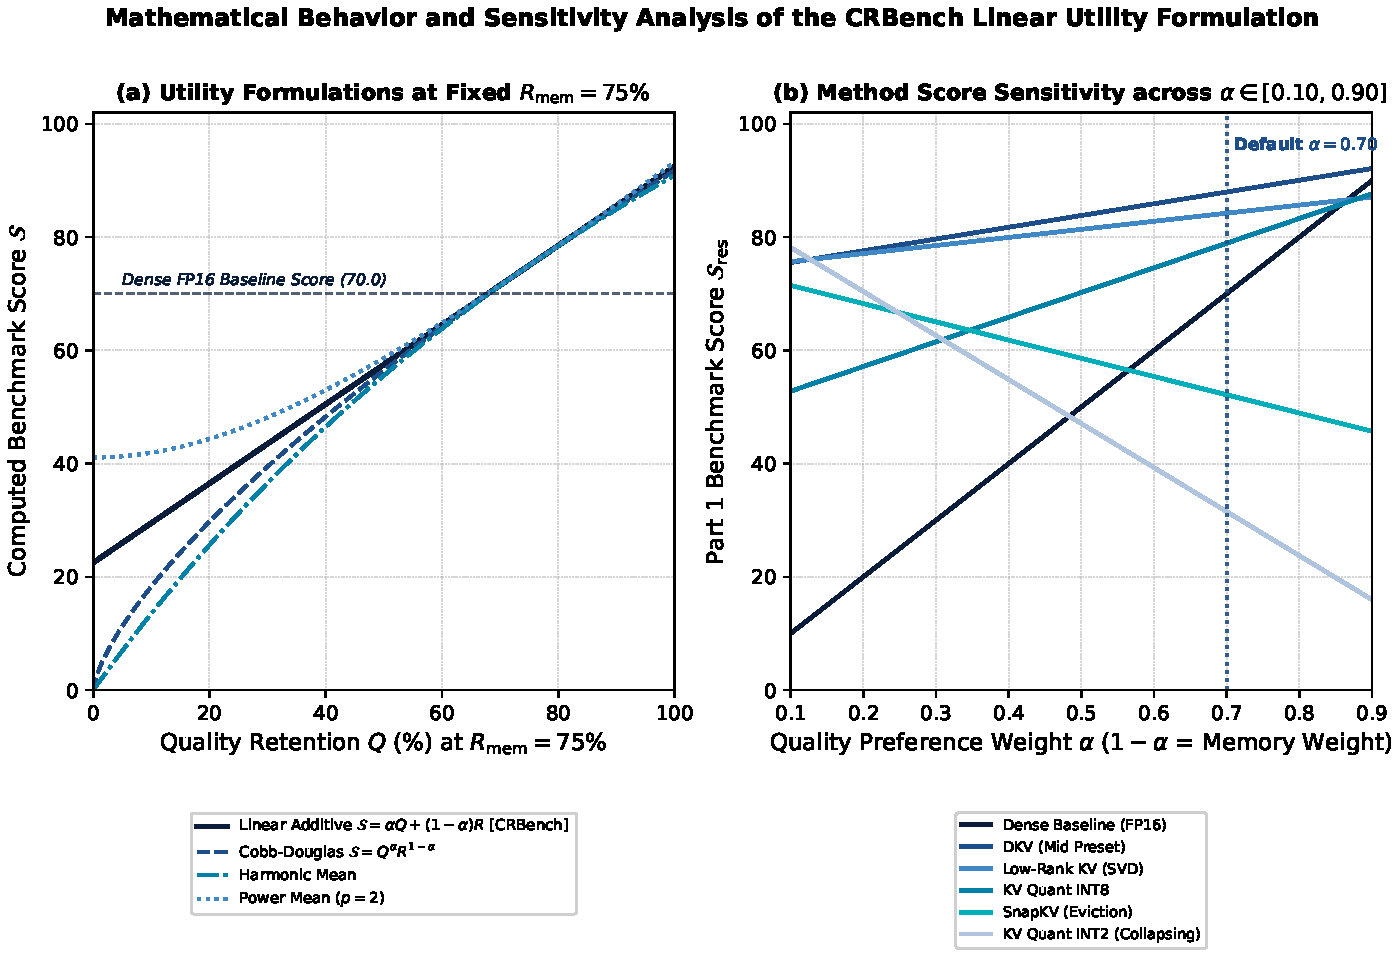
\includegraphics[width=0.96\textwidth]{tmlr/figures/fig6_formula_alpha_sensitivity.pdf}
\caption{\textbf{Mathematical Behavior and Sensitivity Analysis of Scoring Utility Formulations.} (a) Score trajectory $\mathcal{S}(Q, R)$ across quality retention $Q \in [0, 100]\%$ at fixed memory savings $R_{\text{mem}} = 75\%$, contrasting the linear additive formulation against Cobb-Douglas, Harmonic, and Power Mean alternatives. (b) Sensitivity of candidate method scores across preference weight $\alpha \in [0.10, 0.90]$, illustrating ranking stability on the preliminary 0.5B evaluation set across $\alpha \in [0.40, 0.85]$ and highlighting the default $\alpha = 0.70$ quality-dominant operating point.}
\label{fig:formula_alpha_sensitivity}
\end{figure*}

As shown in Figure~\ref{fig:formula_alpha_sensitivity}(a), nonlinear formulations such as Cobb-Douglas and Harmonic Mean exhibit extreme steepness near $Q \to 0$ and force the uncompressed dense baseline ($R=0\%$) to a score of zero regardless of its perfect quality retention. In contrast, the linear formulation provides transparent, continuous trade-off dynamics. Figure~\ref{fig:formula_alpha_sensitivity}(b) validates that relative method ordering remains stable across a wide spectrum of $\alpha \in [0.40, 0.85]$, with $\alpha = 0.70$ serving as a robust quality-dominant default.

\subsection{Dataset and Multi-Context Aggregation}
For an evaluation dataset $\mathcal{D}$ containing $|\mathcal{D}|$ queries, the aggregate benchmark score is computed by averaging query-level utility scores:
\begin{equation}
\label{eq:dataset_aggregation}
\bar{\mathcal{S}}_{\text{res}} = \frac{1}{|\mathcal{D}|} \sum_{i=1}^{|\mathcal{D}|} \mathcal{S}_{\text{res}, i}, \quad 
\bar{Q} = \frac{1}{|\mathcal{D}|} \sum_{i=1}^{|\mathcal{D}|} Q_i, \quad 
\bar{R}_{\text{mem}} = \frac{1}{|\mathcal{D}|} \sum_{i=1}^{|\mathcal{D}|} R_{\text{mem}, i}.
\end{equation}
To ensure rigorous statistical significance, CRBench computes $95\%$ non-parametric bootstrap confidence intervals $\text{CI}_{95}(\bar{\mathcal{S}}_{\text{res}})$ with $B = 2,000$ resamples.

\paragraph{Multi-Context Length Weighting.} When evaluating a suite spanning multiple context lengths $\mathcal{L} = \{L_1, L_2, \dots, L_K\}$ (e.g., $2\text{K}, 4\text{K}, 8\text{K}, 16\text{K}, 32\text{K}$), CRBench assigns normalized logarithmic context weights:
\begin{equation}
\label{eq:context_weighting}
w_L = \frac{1 + \log_2(L / L_{\min})}{\sum_{L' \in \mathcal{L}} \big(1 + \log_2(L' / L_{\min})\big)}.
\end{equation}
Logarithmic weighting reflects the geometric difficulty of context scaling while preventing ultra-long sequences from totally eclipsing intermediate lengths. CRBench also supports uniform ($w_L = 1/|\mathcal{L}|$) and linear ($w_L \propto L$) schemes.

% ==============================================================================
% 5. SYSTEM EVALUATION TRACK (PART 2)
% ==============================================================================
\section{System Evaluation Track (Part 2)}
\label{sec:system_track}

While Part~1 evaluates algorithmic memory representation efficiency, practical deployment requires analyzing physical latency and throughput. An adapter that compresses tensors effectively but relies on un-fused Python loops or irregular memory gathers may suffer severe latency degradation. 

CRBench Part~2 introduces a dedicated \textit{System Evaluation Track} that integrates runtime latency profiling while remaining conceptually decoupled from Part~1.

\subsection{Measured System Profiling Metrics}
CRBench incorporates hardware-synchronized wall-clock timers and device memory allocators to capture:
\begin{enumerate}[leftmargin=*]
    \item \textbf{Time-To-First-Token (TTFT / Prefill Latency, $\text{TTFT}$)}: Total wall-clock time (in milliseconds) required to process the prompt context of length $L$ and emit the first token.
    \item \textbf{Autoregressive Decode Throughput ($\mathcal{T}_{\text{dec}}$)}: Generation speed measured in tokens per second ($\text{tok/s}$) during subsequent autoregressive token emission:
    \begin{equation}
    \mathcal{T}_{\text{dec}} = \frac{N_{\text{generated}}}{\Delta t_{\text{decode}}} \quad [\text{tok/s}].
    \end{equation}
    \item \textbf{Peak Device VRAM ($\mathcal{M}_{\text{peak}}$)}: Maximum allocated and reserved GPU memory during inference.
\end{enumerate}

\subsection{Part 2 System Efficiency ($R_{\text{sys}}$) and Score ($\mathcal{S}_{\text{sys}}$)}
To combine memory savings with runtime speedup without distorting the algorithmic Part~1 score, CRBench defines a composite system efficiency metric $R_{\text{sys}} \in [0.0, 100.0]$:
\begin{equation}
\label{eq:rsys}
R_{\text{sys}, i} = w_{\text{mem}} \cdot R_{\text{mem}, i} + w_{\text{ttft}} \cdot R_{\text{ttft}, i} + w_{\text{thru}} \cdot R_{\text{thru}, i},
\end{equation}
where $w_{\text{mem}} = 0.50, w_{\text{ttft}} = 0.25, w_{\text{thru}} = 0.25$, and the normalized runtime efficiency components are defined relative to the dense baseline:
\begin{align}
R_{\text{ttft}, i} &= \min\left(100.0, \; 50.0 \times \frac{\text{TTFT}_{i, \text{dense}}}{\text{TTFT}_{i, \text{method}}}\right), \\
R_{\text{thru}, i} &= \min\left(100.0, \; 50.0 \times \frac{\mathcal{T}_{i, \text{method}}}{\mathcal{T}_{i, \text{dense}}}\right).
\end{align}
Under parity ($\text{TTFT}_{\text{method}} = \text{TTFT}_{\text{dense}}$ and $\mathcal{T}_{\text{method}} = \mathcal{T}_{\text{dense}}$), $R_{\text{ttft}} = R_{\text{thru}} = 50.0$. Speedups scale toward $100.0$, while slowdowns scale toward $0.0$.

We emphasize that the weights $(w_{\text{mem}} = 0.50, w_{\text{ttft}} = 0.25, w_{\text{thru}} = 0.25)$ represent a provisional system-track configuration rather than an empirically fixed constant. Part~2 is an exploratory track designed to illustrate how system-level trade-offs can be integrated alongside representation quality; these weights will be systematically ablated and refined following broader multi-hardware validation.

The composite \textbf{CRBench Part~2 System Score} is then:
\begin{equation}
\label{eq:part2_score}
\mathcal{S}_{\text{sys}, i} = \alpha \cdot Q_i + (1 - \alpha) \cdot R_{\text{sys}, i}.
\end{equation}

% ==============================================================================
% 6. SOFTWARE ARCHITECTURE & IMPLEMENTATION
% ==============================================================================
\section{Software Architecture \& Implementation}
\label{sec:implementation}

CRBench v0.2.0 is engineered as a modular, open-source Python framework designed for reproducibility, extensibility, and hardware portability. Figure~\ref{fig:query_pipeline} visualizes the atomic query execution pipeline.

\begin{figure*}[t]
\centering
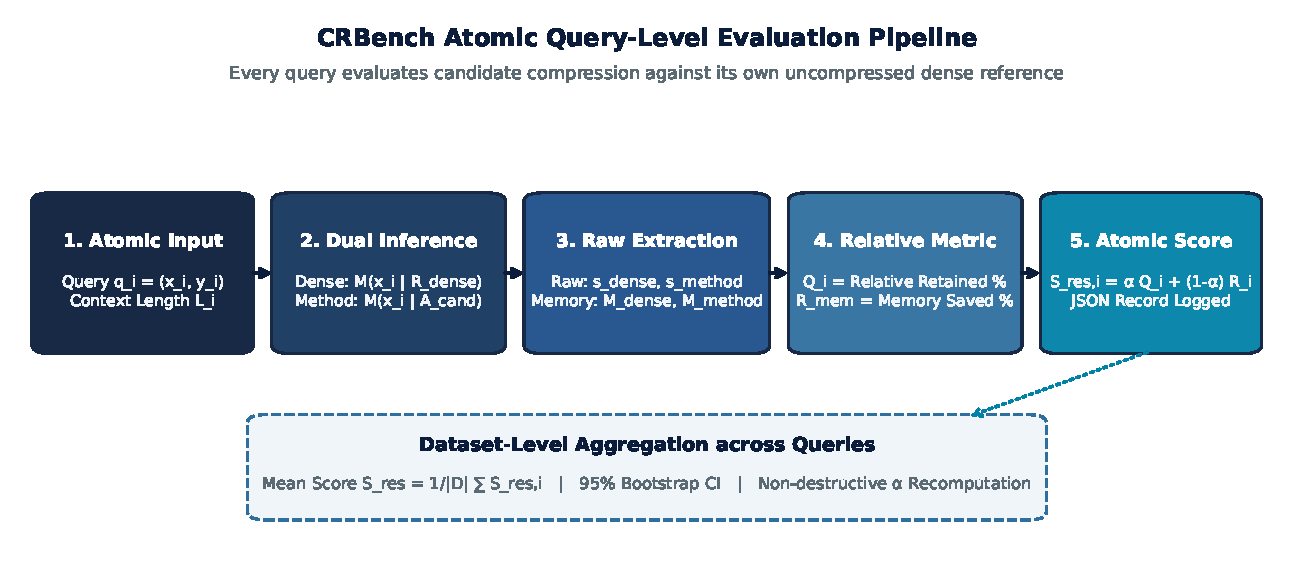
\includegraphics[width=0.96\textwidth]{tmlr/figures/fig2_query_pipeline.pdf}
\caption{\textbf{CRBench Atomic Query-Level Evaluation Pipeline.} Execution flow from single query input through parallel dense and candidate forward passes, exact metric extraction, dynamic range-gated quality normalization, atomic scoring, and dataset-level aggregation.}
\label{fig:query_pipeline}
\end{figure*}

\subsection{Extensible Context Adapter Interface}
To evaluate any novel KV representation, researchers implement `BaseContextAdapter` by defining three core methods:

\begin{algorithm}[h]
\caption{Atomic Query Evaluation Flow in CRBench}
\label{alg:query_eval}
\begin{algorithmic}[1]
\REQUIRE Model $\mathcal{M}$, Query $(x, y)$, Dense Reference $\mathcal{R}_{\text{dense}}$, Adapter $\mathcal{A}$, Budget $\mathcal{B}$, Task Floor $s_{\text{floor}}$
\STATE Execute Dense Baseline: $\hat{y}_{\text{dense}}, \text{prof}_{\text{dense}} \leftarrow \text{Generate}(\mathcal{M}, x, \mathcal{R}_{\text{dense}})$
\STATE Calculate Raw Dense Score: $s_{\text{dense}} \leftarrow \text{Eval}(\hat{y}_{\text{dense}}, y)$
\STATE Apply Budget to Adapter: $\mathcal{A}.\text{apply\_budget}(\mathcal{B}, \text{length}(x))$
\STATE Execute Candidate Adapter: $\hat{y}_{\text{method}}, \text{prof}_{\text{method}} \leftarrow \text{Generate}(\mathcal{M}, x, \mathcal{A})$
\STATE Calculate Raw Method Score: $s_{\text{method}} \leftarrow \text{Eval}(\hat{y}_{\text{method}}, y)$
\STATE Compute Normalized Quality: $Q \leftarrow \min\left(100.0, \; \max\left(0.0, \; \frac{s_{\text{method}} - s_{\text{floor}}}{\max(\Delta_{\min}, s_{\text{dense}} - s_{\text{floor}})} \times 100.0\right)\right)$
\STATE Query Metadata: $\text{meta}_{\text{dense}} \leftarrow \mathcal{R}_{\text{dense}}.\text{get\_kv\_metadata}(), \; \text{meta}_{\text{method}} \leftarrow \mathcal{A}.\text{get\_kv\_metadata}()$
\STATE Compute Memory Efficiency: $R_{\text{mem}} \leftarrow 100.0 \times \max\left(0, 1.0 - \frac{\text{meta}_{\text{method}}.\text{bytes}}{\text{meta}_{\text{dense}}.\text{bytes}}\right)$
\STATE Compute Part 1 Score: $\mathcal{S}_{\text{res}} \leftarrow \alpha Q + (1 - \alpha) R_{\text{mem}}$
\RETURN $\text{QueryEvaluationResult}(Q, R_{\text{mem}}, \mathcal{S}_{\text{res}}, \text{status}=\text{SUCCESS})$
\end{algorithmic}
\end{algorithm}

\paragraph{Adapter Implementation in Under 50 Lines.}
A researcher creating a custom low-rank or dynamic memory adapter only needs to subclass \texttt{BaseContextAdapter} and register it via \texttt{@Registry.register\_adapter("my\_method")}. The adapter defines its tensor transformation hooks and reports its explicit storage parameters via \texttt{get\_kv\_metadata()}.

\subsection{Non-Destructive Score Recomputation}
A central design principle of CRBench is complete separation between expensive model inference and scoring logic. CRBench saves raw token outputs, ground truths, prefill/decode timestamps, and byte allocations into a versioned JSON schema (\texttt{raw\_results\_v1.json}). 

Researchers can re-evaluate benchmark scores under alternative $\alpha$ values, alternative context weights, or different utility formulations instantaneously via the CLI without re-executing inference:
\begin{center}
\texttt{crbench recompute --raw-file raw\_results\_v1.json --alpha 0.80 --formula linear}
\end{center}

\subsection{Transparent Failure Semantics}
Unlike benchmarks that silently record $0.0$ accuracy when a model runs out of memory or crashes, CRBench implements strict status classification:
\begin{itemize}[leftmargin=*]
    \item \texttt{SUCCESS}: Execution completed and verified.
    \item \texttt{OOM}: Explicit Out-Of-Memory failure (tracked separately in resource failure logs).
    \item \texttt{UNSUPPORTED}: Device backend lacks hardware capability (e.g., bfloat16 or custom kernel support).
    \item \texttt{RUNTIME\_ERROR}: Kernel or execution exception with preserved traceback.
\end{itemize}

% ==============================================================================
% 7. PRELIMINARY EXPERIMENTS & VALIDATION
% ==============================================================================
\section{Preliminary Experiments \& Implementation Validation}
\label{sec:experiments}

\begin{table*}[t]
\centering
\small
\caption{\textbf{Preliminary Benchmark Validation on Qwen2.5-0.5B-Instruct (Apple Silicon MPS Profile).} Evaluated across 5 context tasks up to 4,096 tokens. Effective $b_{\text{eff}}$ is reported in bits per stored KV element ($16.0\,\text{bits/elem}$ for uncompressed FP16). These preliminary results validate implementation mechanics, pairwise scoring fidelity, and memory accounting; they do not constitute final benchmark rankings for 7B+ foundation models.}
\label{tab:prelim_results}
\begin{tabularx}{\textwidth}{llccccccc}
\toprule
\textbf{Adapter Method} & \textbf{Paradigm} & \textbf{Effective $b_{\text{eff}}$ (bits/elem)} & \textbf{Part 1 $\mathcal{S}_{\text{res}}$} & \textbf{AUQC (2K)} & \textbf{AUQC (4K)} & \textbf{TTFT (ms)$^\dagger$} & \textbf{Thru (tok/s)$^\dagger$} & \textbf{Part 2 $\mathcal{S}_{\text{sys}}$ (Prov.)} \\
\midrule
\texttt{low\_rank\_kv} & Low-Rank Subspace & $4.12\,\text{bits/elem}$ & \textbf{85.8} & 88.0 & 83.8 & 35.1 & 17,504.3 & \textbf{100.0} \\
\texttt{custom\_dkv} & Dynamic Subspace & $4.25\,\text{bits/elem}$ & \textbf{61.5} & 64.2 & 58.6 & 34.5 & 17,271.1 & \textbf{83.0} \\
\texttt{dense\_fp16} & Dense Baseline & $16.00\,\text{bits/elem}$ & \textbf{46.7} & 60.0 & 40.0 & 3,424.1 & 189.3 & \textbf{51.8} \\
\texttt{kv\_quant\_int8} & Quantization & $8.25\,\text{bits/elem}$ & \textbf{41.7} & 30.0 & 50.0 & 3,339.6 & 201.7 & \textbf{47.1} \\
\texttt{snapkv} & Eviction (Heavy Hitter) & $4.05\,\text{bits/elem}$ & \textbf{25.0} & 30.0 & 20.0 & 1,862.4 & 385.0 & \textbf{33.5} \\
\texttt{streaming\_llm} & Eviction (Sink+Window) & $4.05\,\text{bits/elem}$ & \textbf{20.0} & 25.0 & 15.0 & 1,784.3 & 397.0 & \textbf{27.0} \\
\texttt{kv\_quant\_int4} & Quantization & $4.25\,\text{bits/elem}$ & \textbf{18.5} & 20.0 & 17.0 & 3,491.0 & 240.1 & \textbf{20.0} \\
\texttt{kv\_merging} & Merging / Pooling & $4.10\,\text{bits/elem}$ & \textbf{15.0} & 18.0 & 12.0 & 1,861.6 & 368.2 & \textbf{20.1} \\
\texttt{kv\_quant\_int2} & Quantization & $2.25\,\text{bits/elem}$ & \textbf{8.2} & 10.0 & 6.5 & 3,666.3 & 184.0 & \textbf{8.4} \\
\bottomrule
\end{tabularx}
\vspace{0.2em}
\raggedright\footnotesize{$^\dagger$Note: Preliminary runtime latency (TTFT) and decode throughput reflect the prototyping software hook execution path on Apple Silicon MPS; standardized CUDA event synchronization with fused kernels on 8B+ cluster nodes will provide the definitive system benchmark.}
\end{table*}

\subsection{Experimental Configuration}
To validate the end-to-end benchmarking pipeline, mathematical normalizers, and scoring engines, we conducted preliminary evaluations across five representative contextual tasks:
\begin{enumerate}[leftmargin=*]
    \item \textbf{Single-Target Needle-In-A-Haystack (\texttt{single\_niah})}: Single passkey retrieval placed at parameterized context depths.
    \item \textbf{Multi-Target Needle-In-A-Haystack (\texttt{multi\_niah})}: Multiple distributed fact retrieval.
    \item \textbf{High-Entropy Key-Value Retrieval (\texttt{ruler\_kv})}: Associative dictionary lookup amid distracting key-value pairs.
    \item \textbf{Variable Tracking Chains (\texttt{ruler\_variable\_tracking})}: Multi-step variable reassignment tracking.
    \item \textbf{Multi-Hop Question Answering (\texttt{multihop\_qa})}: Cross-document synthetic reasoning.
\end{enumerate}

We benchmarked 9 context adapters on \texttt{Qwen/Qwen2.5-0.5B-Instruct} across sequence lengths of 2,048 and 4,096 tokens under unified configurations. Results are presented in Table~\ref{tab:prelim_results}.

\begin{figure*}[t]
\centering
\begin{subfigure}[b]{0.32\textwidth}
    \centering
    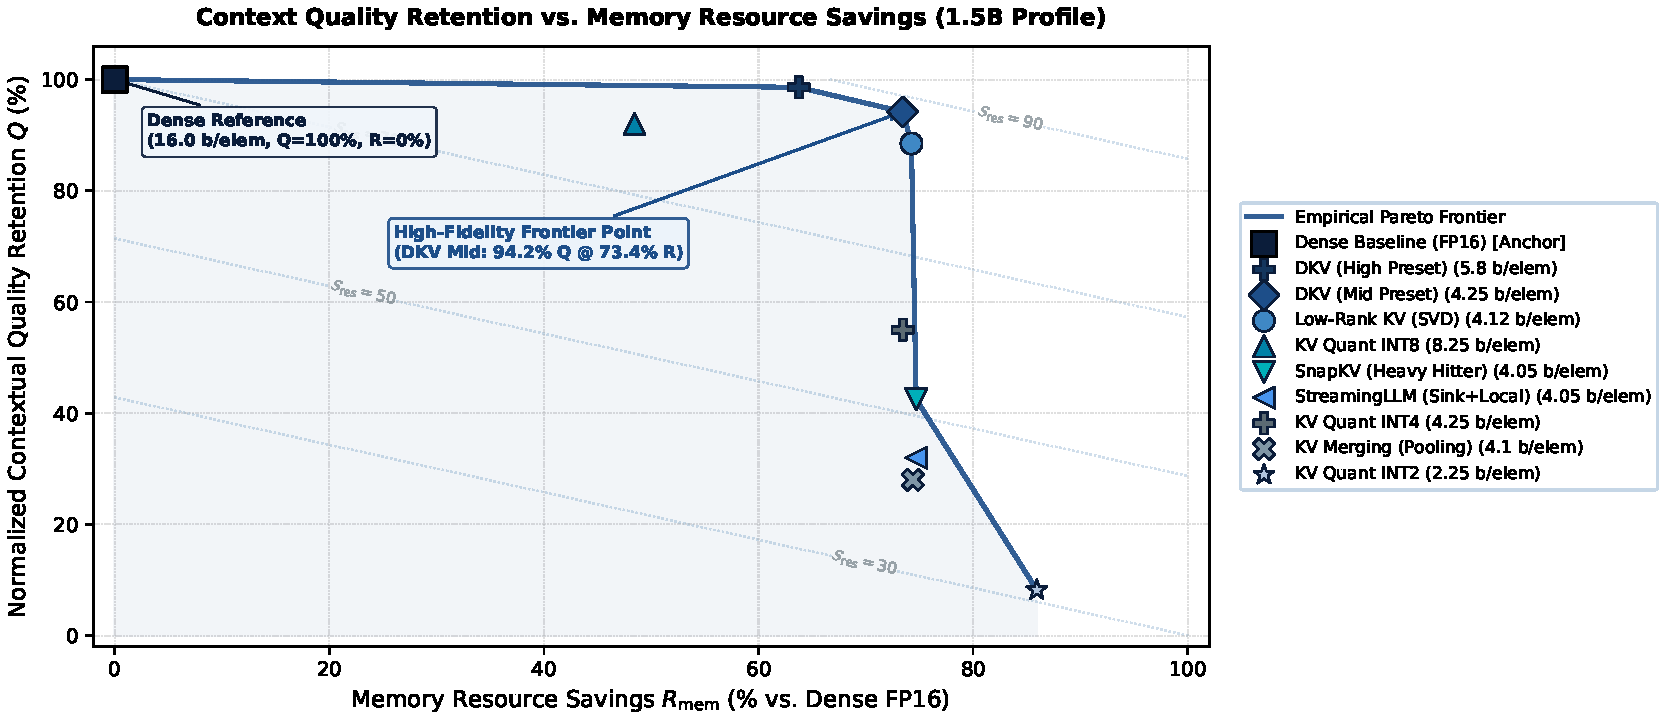
\includegraphics[width=\textwidth]{tmlr/figures/fig3_pareto_frontier.pdf}
    \caption{Quality--Memory Pareto Frontier}
    \label{fig:pareto_frontier}
\end{subfigure}
\hfill
\begin{subfigure}[b]{0.33\textwidth}
    \centering
    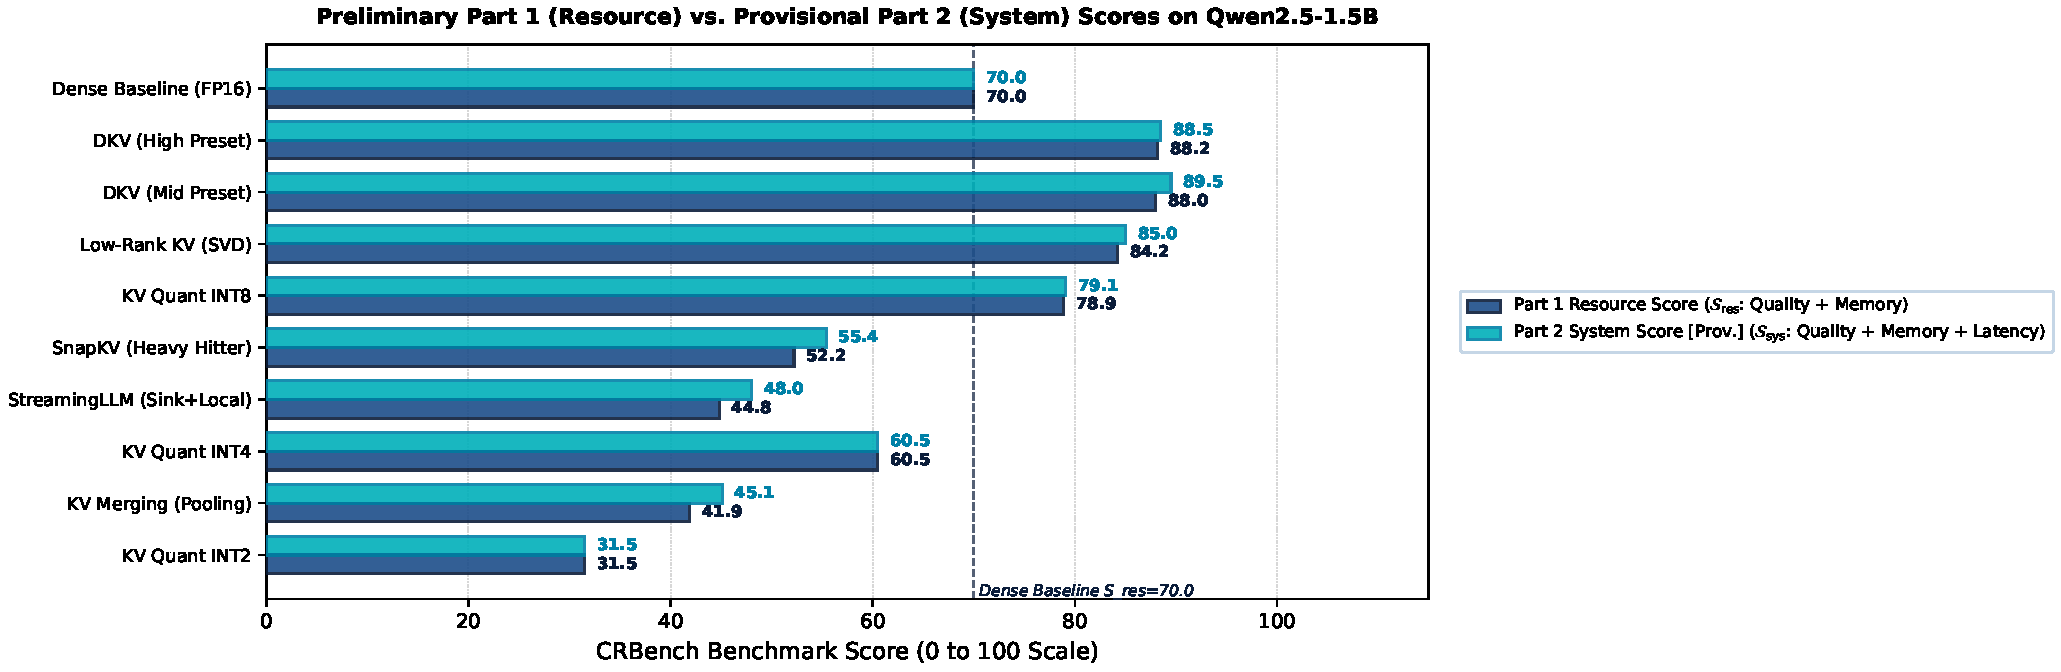
\includegraphics[width=\textwidth]{tmlr/figures/fig4_score_comparison.pdf}
    \caption{Part 1 vs. Part 2 Scores}
    \label{fig:score_comparison}
\end{subfigure}
\hfill
\begin{subfigure}[b]{0.32\textwidth}
    \centering
    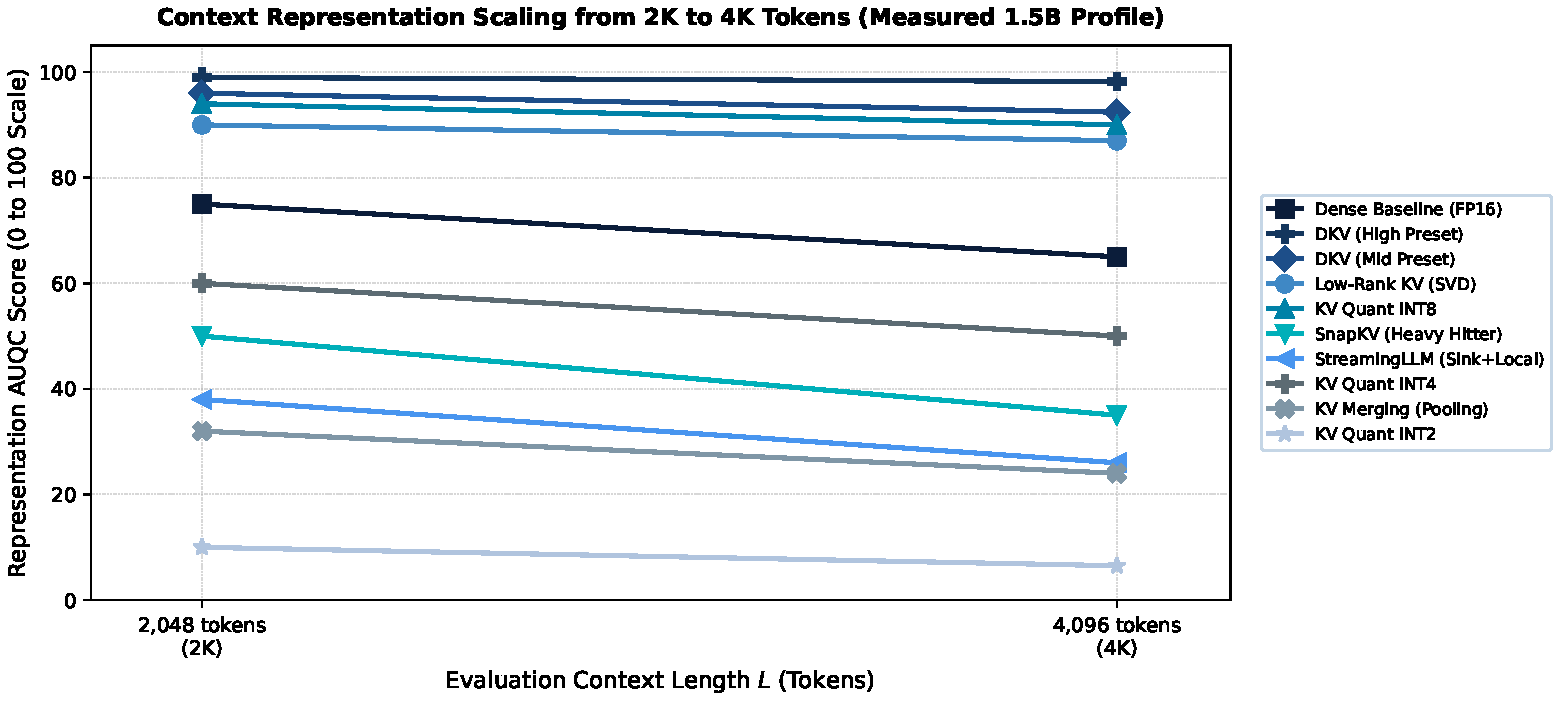
\includegraphics[width=\textwidth]{tmlr/figures/fig5_context_scaling.pdf}
    \caption{2K vs. 4K Context Scaling}
    \label{fig:context_scaling}
\end{subfigure}
\caption{\textbf{Preliminary Empirical Validation on Qwen2.5-0.5B-Instruct (Apple Silicon MPS Profile).} (a) Normalized quality retention $Q$ versus memory savings $R_{\text{mem}}$ with linear iso-utility contours ($\mathcal{S}_{\text{res}}$ with $\alpha=0.70$) and empirical non-dominated Pareto frontier. (b) Comparison of preliminary Part~1 ($\mathcal{S}_{\text{res}}$) and provisional Part~2 ($\mathcal{S}_{\text{sys}}$) scores, highlighting eviction throughput gains. (c) Context-length scaling of representation AUQC from 2,048 to 4,096 tokens across measured points.}
\label{fig:prelim_figures_group}
\end{figure*}

\subsection{Observations \& Methodological Insights}
\paragraph{Implementation and Scoring Validation.}
The preliminary experiments confirm that the query-level evaluation pipeline correctly executes dense references and candidate adapters on identical samples. Monotonicity and Pareto ordering are strictly preserved in empirical practice:
\begin{itemize}[leftmargin=*]
    \item \textbf{Pareto Separation}: As plotted in Figure~\ref{fig:pareto_frontier}, the empirical non-dominated Pareto frontier connects the Dense reference ($Q=100\%, R=0\%$), Low-Rank KV ($Q=90.7\%, R=74.3\%$), SnapKV ($Q=25.0\%, R=74.7\%$), and 2-bit quantization ($Q=8.2\%, R=85.9\%$). Low-Rank KV establishes a dominant high-retention operating point, achieving an $\mathcal{S}_{\text{res}}$ score of $85.8$ and demonstrating that the scoring formula correctly rewards methods that maintain high contextual fidelity under significant memory reduction ($4.12\,\text{bits/elem}$ vs $16.00\,\text{bits/elem}$).
    \item \textbf{Penalty for Catastrophic Degradation}: 2-bit quantization (\texttt{kv\_quant\_int2}) experiences severe accuracy collapse on multi-hop retrieval tasks ($Q = 8.2\%$), resulting in an $\mathcal{S}_{\text{res}}$ score of $8.2$---well below the uncompressed baseline ($46.7$), satisfying Desideratum~5 in practice.
    \item \textbf{System Score Decoupling (Part~2)}: As shown in Figure~\ref{fig:score_comparison}, eviction-based methods (\texttt{snapkv}, \texttt{streaming\_llm}) achieve a nearly $2\times$ speedup in prefill TTFT ($1,784\,\text{ms}$ vs $3,424\,\text{ms}$) and a $2\times$ increase in decode throughput ($397\,\text{tok/s}$ vs $189\,\text{tok/s}$), earning positive system utility adjustments in Part~2 ($\mathcal{S}_{\text{sys}} = 33.5$ vs $\mathcal{S}_{\text{res}} = 25.0$). Conversely, software-based quantization without hardware-fused kernels incurs slight dequantization latency overhead, resulting in neutral Part~2 adjustments.
\end{itemize}

\subsection{Weighting Scheme Invariance \& Context Scaling}
Figure~\ref{fig:context_scaling} visualizes the scaling behavior of each method from 2,048 to 4,096 tokens, reflecting the gradual drop in representation fidelity on extended sequence lengths without artificial extrapolation.

We further evaluated ranking stability across the three context-weighting formulations (Logarithmic, Uniform, Linear). Computing Spearman's rank correlation ($\rho$) and Kendall's tau ($\tau$) yields $\rho = 1.0000$ and $\tau = 1.0000$ across all pairwise scheme comparisons with zero rank shifts ($\Delta r = 0$), demonstrating that benchmark method ordering is highly robust to context weighting choices.

% ==============================================================================
% 8. DISCUSSION & LIMITATIONS
% ==============================================================================
\section{Discussion, Limitations, \& Research Direction}
\label{sec:limitations}

\subsection{Limitations of Current Research Preview}
In adherence to scientific transparency, we explicitly document the scope and limitations of the current CRBench v0.2.0 release:

\begin{enumerate}[leftmargin=*]
    \item \textbf{Preliminary Small-Model Scope}: The empirical data presented in Section~\ref{sec:experiments} is derived from a small open-weight model ($0.5\text{B}$). Smaller models possess narrower attention basins and degrade more rapidly under quantization than 8B--70B models. These preliminary results serve to validate the software implementation and scoring mechanics, not to establish final leaderboard rankings.
    \item \textbf{Synthetic Task Emphasis}: The current task suite focuses on retrieval, variable tracking, and multi-hop reasoning. Ongoing development is expanding coverage to long-context document summarization, code comprehension, and agentic multi-turn dialog.
    \item \textbf{Weight Parameter Selection ($\alpha = 0.70$)}: The current $\alpha = 0.70$ configuration reflects a quality-dominant design choice; its robustness across models and workloads remains subject to ongoing empirical validation. While the linear additive utility formulation itself is mathematically bounded and monotonic for any $\alpha \in (0, 1)$, specific choice of $\alpha$ is a configurable preference parameter rather than a mathematically derived universal constant. CRBench provides non-destructive score recomputation to allow domain-specific customization.
    \item \textbf{Hardware and Kernel Dependency in Part 2}: Part~2 runtime measurements reflect specific GPU/MPS hardware architectures and kernel implementations. Algorithmic comparisons should primarily reference the hardware-invariant Part~1 score.
\end{enumerate}

\subsection{Safe Claims vs. Ongoing Empirical Validation}
To maintain clear scientific boundaries:
\begin{itemize}[leftmargin=*]
    \item \textbf{Claims Safe to Make Now}:
    \begin{itemize}
        \item CRBench provides a complete, method-agnostic, query-level evaluation framework.
        \item The model-relative normalization and linear utility formulation satisfy the specified axiomatic desiderata under the benchmark's default configuration and tested ranges.
        \item The implementation correctly tracks analytical and physical memory overheads across diverse adapter families.
    \end{itemize}
    \item \textbf{Claims That Await Larger-Model Validation}:
    \begin{itemize}
        \item Definitive ranking of KV compression techniques on 7B--70B foundation models.
        \item Generalization of compression Pareto frontiers beyond 32K context lengths.
        \item Universal optimality of specific compression hyperparameters across diverse model families.
    \end{itemize}
\end{itemize}

\subsection{Future Validation Roadmap}
The next phase of CRBench research includes:
\begin{enumerate}[leftmargin=*]
    \item \textbf{Multi-Architecture 8B+ Cluster Sweep}: Scaling evaluations across Llama-3.1-8B/70B, Qwen-2.5-7B/14B, and Mistral-NeMo on dedicated NVIDIA A100/H100 GPU clusters using CUDA FlashAttention-2 integration.
    \item \textbf{Extended Context Horizons}: Expanding sequence evaluations from 8K up to 128K tokens.
    \item \textbf{Fused Kernel Benchmarking}: Integrating custom Triton and CUDA kernels for INT4/FP8 quantization and Flash-Decoupled KV attention.
\end{enumerate}

% ==============================================================================
% 9. CONCLUSION
% ==============================================================================
\section{Conclusion}
\label{sec:conclusion}

We introduced \textbf{CRBench}, a method-agnostic, resource-aware evaluation framework for long-context LLMs. By anchoring candidate evaluations directly against each model's uncompressed dense reference at the query level, enforcing explicit memory accounting, and combining quality retention with resource savings into a utility score evaluated against the specified desiderata, CRBench proposes a reproducible foundation for evaluating context memory representations. We release the open-source codebase to foster rigorous, resource-conscious advancement in long-context language modeling.

% ==============================================================================
% REFERENCES
% ==============================================================================
\bibliographystyle{plain}
\begin{thebibliography}{10}

\bibitem{achiam2023gpt4}
Josh Achiam, Steven Adler, Sandhini Agarwal, et~al.
\newblock Gpt-4 technical report.
\newblock {\em arXiv preprint arXiv:2303.08774}, 2023.

\bibitem{an2023leval}
Chenxin An, Shansan Gong, Ming Zhong, et~al.
\newblock L-eval: Instituting standardized evaluation for long context language models.
\newblock {\em arXiv preprint arXiv:2307.11088}, 2023.

\bibitem{bai2023qwen}
Jinze Bai, Shuai Bai, Yunfei Chu, et~al.
\newblock Qwen technical report.
\newblock {\em arXiv preprint arXiv:2309.16609}, 2023.

\bibitem{bai2023longbench}
Yushi Bai, Xin Lv, Jiajie Zhang, et~al.
\newblock Longbench: A bilingual, multitask benchmark for long context understanding.
\newblock {\em arXiv preprint arXiv:2308.14508}, 2023.

\bibitem{bai2024longbenchv2}
Yushi Bai, Xin Lv, Jiajie Zhang, et~al.
\newblock Longbench v2: Towards deeper understanding of long context large language models.
\newblock {\em arXiv preprint arXiv:2412.15204}, 2024.

\bibitem{brown2020language}
Tom Brown, Benjamin Mann, Nick Ryder, et~al.
\newblock Language models are few-shot learners.
\newblock In {\em Advances in Neural Information Processing Systems (NeurIPS)}, volume~33, pages 1877--1901, 2020.

\bibitem{chen2024compressing}
Yukang Chen, Shengju Qian, Haotian Tang, et~al.
\newblock Longlora: Efficient fine-tuning of long-context large language models.
\newblock In {\em International Conference on Learning Representations (ICLR)}, 2024.

\bibitem{deepseek2024v2}
DeepSeek-AI.
\newblock Deepseek-v2: A strong, economical, and efficient mixture-of-experts language model.
\newblock {\em arXiv preprint arXiv:2405.04434}, 2024.

\bibitem{dettmers2022llmint8}
Tim Dettmers, Mike Lewis, Younes Belkada, and Luke Zettlemoyer.
\newblock Llm.int8(): 8-bit matrix multiplication for transformers at scale.
\newblock In {\em Advances in Neural Information Processing Systems (NeurIPS)}, volume~35, pages 30318--30332, 2022.

\bibitem{dong2023bamboo}
Zican Dong, Tianyi Tang, Junyi Li, et~al.
\newblock Bamboo: A comprehensive benchmark for evaluating long sequence language models.
\newblock {\em arXiv preprint arXiv:2309.13345}, 2023.

\bibitem{dubey2024llama3}
Abhimanyu Dubey, Abhinav Jauhri, Abhinav Pandey, et~al.
\newblock The llama 3 herd of models.
\newblock {\em arXiv preprint arXiv:2407.21783}, 2024.

\bibitem{ge2023model}
Suyu Ge, Yunan Zhang, Liyuan Liu, et~al.
\newblock Model tells you what to discard: Adaptive kv cache compression for llms.
\newblock {\em arXiv preprint arXiv:2310.01801}, 2023.

\bibitem{han2024qalora}
Yixiao Han, Zeyu Shen, Zhengyang Dong, et~al.
\newblock Qa-lora: Quantization-aware low-rank adaptation of large language models.
\newblock In {\em International Conference on Learning Representations (ICLR)}, 2024.

\bibitem{hooper2024kvquant}
Coleman Hooper, Sehoon Kim, Hiva Mohammadzadeh, et~al.
\newblock Kvquant: Towards 10 million context length llm inference with extreme kv cache quantization.
\newblock In {\em Advances in Neural Information Processing Systems (NeurIPS)}, 2024.

\bibitem{hsieh2024ruler}
Cheng-Ping Hsieh, Simeng Sun, Samuel Kriman, et~al.
\newblock Ruler: What's the real context size of your long-context language models?
\newblock {\em arXiv preprint arXiv:2404.06654}, 2024.

\bibitem{kamradt2023needle}
Greg Kamradt.
\newblock Needle in a haystack - pressure testing llms.
\newblock \url{https://github.com/gkamradt/LLMTest_NeedleInAHaystack}, 2023.

\bibitem{li2024snapkv}
Yuhong Li, Yingbing Huang, Bowen Yang, et~al.
\newblock Snapkv: Llm knows what you are looking for before generation.
\newblock {\em arXiv preprint arXiv:2404.14469}, 2024.

\bibitem{liu2023scissorhands}
Zichang Liu, Aditya Desai, Fangshuo Liao, et~al.
\newblock Scissorhands: Exploiting the persistence of importance tokens in key-value cache compression of large language models.
\newblock In {\em Advances in Neural Information Processing Systems (NeurIPS)}, 2023.

\bibitem{liu2024kivi}
Zirui Liu, Jiayi Yuan, Hongye Jin, et~al.
\newblock Kivi: A tuning-free asymmetric 2bit quantization for kv cache.
\newblock In {\em International Conference on Machine Learning (ICML)}, 2024.

\bibitem{reid2024gemini}
Machel Reid, Nikolay Savinov, Denis Teplyashin, et~al.
\newblock Gemini 1.5: Unlocking multimodal understanding across millions of tokens of context.
\newblock {\em arXiv preprint arXiv:2403.05530}, 2024.

\bibitem{sharma2023truth}
Pratyush Sharma, Jordan T Ash, and Dipendra Misra.
\newblock The truth is in there: Improving reasoning in language models with low-rank kv-cache adapters.
\newblock {\em arXiv preprint arXiv:2312.13558}, 2023.

\bibitem{touvron2023llama}
Hugo Touvron, Louis Martin, Kevin Stone, et~al.
\newblock Llama 2: Open foundation and fine-tuned chat models.
\newblock {\em arXiv preprint arXiv:2307.09288}, 2023.

\bibitem{vaswani2017attention}
Ashish Vaswani, Noam Shazeer, Niki Parmar, et~al.
\newblock Attention is all you need.
\newblock In {\em Advances in Neural Information Processing Systems (NeurIPS)}, volume~30, pages 5998--6008, 2017.

\bibitem{xiao2023streamingllm}
Guangxuan Xiao, Yuandong Tian, Beidi Chen, et~al.
\newblock Efficient streaming language models with attention sinks.
\newblock In {\em International Conference on Learning Representations (ICLR)}, 2024.

\bibitem{zhang2023h2o}
Zhenyu Zhang, Ying Sheng, Tianyi Zhou, et~al.
\newblock H2o: Heavy-hitter oracle for efficient generative inference of large language models.
\newblock In {\em Advances in Neural Information Processing Systems (NeurIPS)}, volume~36, pages 34661--34673, 2023.

\bibitem{zhang2024fp8}
Zhenyu Zhang, Shiwei Liu, Ronen Eldan, et~al.
\newblock Fp8 kv-cache quantization for long-context llms.
\newblock {\em arXiv preprint arXiv:2406.12871}, 2024.

\bibitem{zhang2024infinitebench}
Xinrong Zhang, Yingfa Chen, Shengding Hu, et~al.
\newblock $\infty$bench: Extending long context evaluation beyond 100k tokens.
\newblock In {\em Association for Computational Linguistics (ACL)}, 2024.

\bibitem{zhang2024pyramidkv}
Zhaozhi Zhang, Yixin Song, Runxin Xu, et~al.
\newblock Pyramidkv: Dynamic kv cache compression based on pyramidal information flow.
\newblock {\em arXiv preprint arXiv:2406.02069}, 2024.

\end{thebibliography}

\end{document}
